\clearpage
\section{Результаты вычислительного эксперимента}
	Архитектуры нейронных сетей, а также модификация процедуры обучения, описанные в пунктах 1.4.3 и 1.4.4 были реализованы в виде комплекса программ на языке Python с помощью библиотеки для глубокого обучения PyTorch. Использованные версии программных пакетов указаны в Приложении 1. Обучение проводилось на наборе данных Berea.
	
	\subsection{Набор данных Berea}
		Исходные данные - изображение компьютерной томографии песчаника, объёмом $400^3$ вокселей, бинарно сегментированная на породу и поры, в формате TIFF. Разрешение томограммы равно 3 микрометрам. Для обучения сетей из этого кубика был вырезан набор кубиков размером $64^3$ вокселей, с перекрытием в 16 вокселей (всего 10648 различных образцов размера $64^3$), они и представили собой обучающую выборку. Оригинальный образец размером $400^3$ вокселей представлен на (Рис. \ref{5-full-berea}). Некоторые примеры из получившейся обучающей выборки представлены в (Таб. \ref{5-berea64}).
		
		\begin{figure}[h!]
			\centering{\includegraphics[width=0.6\linewidth]{5-results/berea/original}}
			\caption{Оригинальный образец}
			\label{5-full-berea}
		\end{figure}
	
		\begin{table}[h!]
			\begin{center}
				\begin{tabular}{p{5cm} p{5cm} p{5cm}}
					\toprule
					\includegraphics[width=0.9\linewidth]{5-results/berea/berea_1}
					&
					\includegraphics[width=0.9\linewidth]{5-results/berea/berea_2}
					&
					\includegraphics[width=0.9\linewidth]{5-results/berea/berea_3}
					\\
					\includegraphics[width=0.9\linewidth]{5-results/berea/berea_4}
					&
					\includegraphics[width=0.9\linewidth]{5-results/berea/berea_5}
					&
					\includegraphics[width=0.9\linewidth]{5-results/berea/berea_6}
					\\
					\bottomrule
				\end{tabular}
				\caption{Примеры из обучающей выборки}
				\label{5-berea64}
			\end{center}
		\end{table}
	\subsection{Обучение нейросети}
		Было проведено обучение нейросети со следующими параметрами (число сверточных фильтров указано для первого слоя):
		\begin{table}[h!]
			\begin{center}
				\begin{tabular}{|c|c|c|c|}
					\hline
					Число фильтров G, D & Размерность z & Размер пакета & Начальный LR \\
					\hline
					64, 32 & 512 & 64 & 2e-4 \\
					\hline
				\end{tabular}
				\caption{Гиперпараметры нейросети и процесса обучения}
			\end{center}
		\end{table}
		
		Графики функций ошибок сетей генератора и дискриминатора, а также графики сходимостей функционалов Минковского в процессе обучения приведены на (Рис. \ref{loss-plot}, \ref{V-plot}, \ref{S-plot}, \ref{B-plot}, \ref{Xi-plot}).
		
		\begin{figure}[h!]
			\centering{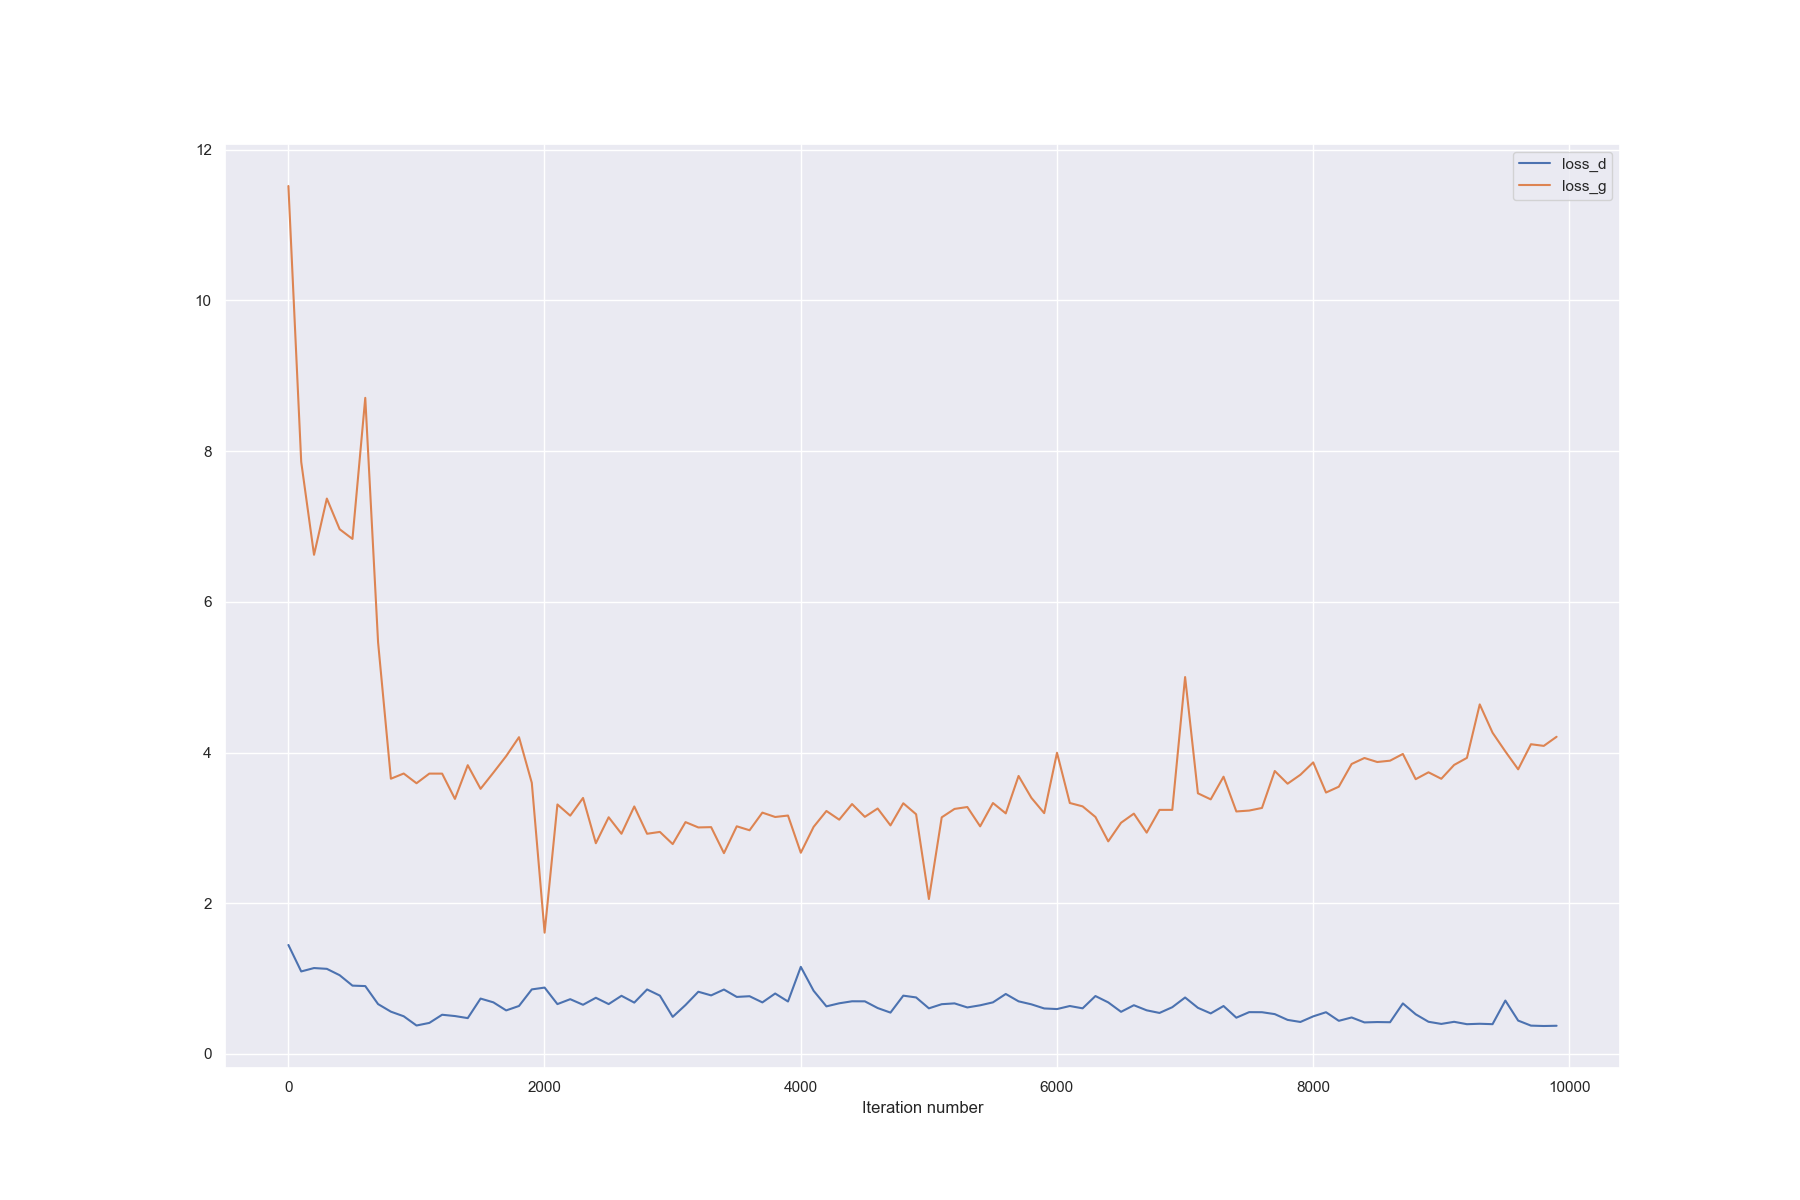
\includegraphics[width=0.95\linewidth]{5-results/experiment/loss_plot}}
			\caption{График функций ошибок сетей дискриминатора и генератора}
			\label{loss-plot}
		\end{figure}
	
		\begin{figure}[h!]
			\centering{\includegraphics[width=0.95\linewidth]{5-results/experiment/minkowski_V_plot}}
			\caption{График сходимости функционала Минковского $V$}
			\label{V-plot}
		\end{figure}
		
		\begin{figure}[h!]
			\centering{\includegraphics[width=0.95\linewidth]{5-results/experiment/minkowski_S_plot}}
			\caption{График сходимости функционала Минковского $S$}
			\label{S-plot}
		\end{figure}
	
		\begin{figure}[h!]
			\centering{\includegraphics[width=0.95\linewidth]{5-results/experiment/minkowski_B_plot}}
			\caption{График сходимости функционала Минковского $B$}
			\label{B-plot}
		\end{figure}
	
		\begin{figure}[h!]
			\centering{\includegraphics[width=0.95\linewidth]{5-results/experiment/minkowski_Xi_plot}}
			\caption{График сходимости функционала Минковского $\xi$}
			\label{Xi-plot}
		\end{figure}	
		
	
	\subsection{Реконструкции размера $64^3$}
		\subsubsection{Примеры}
			Примеры реконструкции размера $64^3$, приведены в (Таб. \ref{5-gen-64}). Дополнительные примеры реконструкций приведены в Приложении 2 (Таб. \ref{8-gen-64})
			
			\begin{table}[h!]
				\begin{center}
					\begin{tabular}{p{5cm} p{5cm} p{5cm}}
						\toprule
						\includegraphics[width=1\linewidth]{5-results/analysis_64/generated/1}
						&
						\includegraphics[width=1\linewidth]{5-results/analysis_64/generated/2}
						&
						\includegraphics[width=1\linewidth]{5-results/analysis_64/generated/3}
						\\
						\includegraphics[width=1\linewidth]{5-results/analysis_64/generated/4}
						&
						\includegraphics[width=1\linewidth]{5-results/analysis_64/generated/5}
						&
						\includegraphics[width=1\linewidth]{5-results/analysis_64/generated/6}
						\\
						\includegraphics[width=1\linewidth]{5-results/analysis_64/generated/7}
						&
						\includegraphics[width=1\linewidth]{5-results/analysis_64/generated/8}
						&
						\includegraphics[width=1\linewidth]{5-results/analysis_64/generated/9}
						\\
						\bottomrule
					\end{tabular}
					\caption{Примеры реконструкции 64x64x64}
					\label{5-gen-64}
				\end{center}
			\end{table} 
		
		\subsubsection{Анализ}
			Было реконструировано 1000 образцов размера $64^3$. На основе этого набора были получены распределения интересующих функционалов Минковского. Так же, используя предоставленную обученную сеть \cite{Mosser}, было реконструировано 1000 образцов того же размера для сравнения распределений функционалов. Графики полученных распределений (вместе с соответствующим распределением на обучающей выборке) приведены на (Рис. \ref{5-dist-V-64}, \ref{5-dist-S-64}, \ref{5-dist-B-64}, \ref{5-dist-Xi-64}). Также были рассчитаны двухточечная функция вероятности и соответствующая функция корреляции для реконструированных образцов, образцов, полученных с помощью предобученной сети \cite{Mosser} и образцов из обучающей выборки. Их графики приведены на (Рис. \ref{5-prob-64}, \ref{5-corr-64}).
			
			\begin{figure}[h]
				\begin{minipage}[h]{0.49\linewidth}
					\centering{\includegraphics[width=1\linewidth]{5-results/analysis_64/V_exp} \\ Обученная сеть}
				\end{minipage}
				\hfill
				\begin{minipage}[h]{0.49\linewidth}
					\centering{\includegraphics[width=1\linewidth]{5-results/analysis_64/V_paper} \\ Mosser et al. \cite{Mosser}}
				\end{minipage}
				\caption{Распределения функционала Минковского $V$ для реконструкций размера $64^3$}
				\label{5-dist-V-64}
			\end{figure}
		
			\begin{figure}[h]
				\begin{minipage}[h]{0.49\linewidth}
					\centering{\includegraphics[width=1\linewidth]{5-results/analysis_64/S_exp} \\ Обученная сеть}
				\end{minipage}
				\hfill
				\begin{minipage}[h]{0.49\linewidth}
					\centering{\includegraphics[width=1\linewidth]{5-results/analysis_64/S_paper} \\ Mosser et al. \cite{Mosser}}
				\end{minipage}
				\caption{Распределения функционала Минковского $S$ для реконструкций размера $64^3$}
				\label{5-dist-S-64}
			\end{figure}
		
			\begin{figure}[h]
				\begin{minipage}[h]{0.49\linewidth}
					\centering{\includegraphics[width=1\linewidth]{5-results/analysis_64/B_exp} \\ Обученная сеть}
				\end{minipage}
				\hfill
				\begin{minipage}[h]{0.49\linewidth}
					\centering{\includegraphics[width=1\linewidth]{5-results/analysis_64/B_paper} \\ Mosser et al. \cite{Mosser}}
				\end{minipage}
				\caption{Распределения функционала Минковского $B$ для реконструкций размера $64^3$}
				\label{5-dist-B-64}
			\end{figure}
		
			\begin{figure}[h]
				\begin{minipage}[h]{0.49\linewidth}
					\centering{\includegraphics[width=1\linewidth]{5-results/analysis_64/Xi_exp} \\ Обученная сеть}
				\end{minipage}
				\hfill
				\begin{minipage}[h]{0.49\linewidth}
					\centering{\includegraphics[width=1\linewidth]{5-results/analysis_64/Xi_paper} \\ Mosser et al. \cite{Mosser}}
				\end{minipage}
				\caption{Распределения функционала Минковского $\xi$ для реконструкций размера $64^3$}
				\label{5-dist-Xi-64}
			\end{figure}
		
			\begin{figure}[h]
				\begin{minipage}[h]{0.49\linewidth}
					\centering{\includegraphics[width=1\linewidth]{5-results/analysis_64/prob_exp} \\ Обученная сеть}
				\end{minipage}
				\hfill
				\begin{minipage}[h]{0.49\linewidth}
					\centering{\includegraphics[width=1\linewidth]{5-results/analysis_64/prob_paper} \\ Mosser et al. \cite{Mosser}}
				\end{minipage}
				\caption{Двухточечная функция вероятности для реконструкций размера $64^3$}
				\label{5-prob-64}
			\end{figure}
		
			\begin{figure}[h]
				\begin{minipage}[h]{0.49\linewidth}
					\centering{\includegraphics[width=1\linewidth]{5-results/analysis_64/corr_exp} \\ Обученная сеть}
				\end{minipage}
				\hfill
				\begin{minipage}[h]{0.49\linewidth}
					\centering{\includegraphics[width=1\linewidth]{5-results/analysis_64/corr_paper} \\ Mosser et al. \cite{Mosser}}
				\end{minipage}
				\caption{Двухточечная функция корреляции для реконструкций размера $64^3$}
				\label{5-corr-64}
			\end{figure}
	
	\subsection{Реконструкции размера $200^3$}
		\subsubsection{Примеры}
			Примеры реконструкции размера $200^3$, приведены в (Таб. \ref{5-gen-200}). Дополнительные примеры реконструкций приведены в Приложении 2.
		
			\begin{table}[h!]
				\begin{center}
					\begin{tabular}{p{5cm} p{5cm} p{5cm}}
						\toprule
						\includegraphics[width=1\linewidth]{5-results/analysis_200/generated/1}
						&
						%\includegraphics[width=1\linewidth]{5-results/analysis_200/generated/2}
						&
						%\includegraphics[width=1\linewidth]{5-results/analysis_200/generated/3}
						\\
						%\includegraphics[width=1\linewidth]{5-results/analysis_200/generated/4}
						&
						%\includegraphics[width=1\linewidth]{5-results/analysis_200/generated/5}
						&
						%\includegraphics[width=1\linewidth]{5-results/analysis_200/generated/6}
						\\
						%\includegraphics[width=1\linewidth]{5-results/analysis_200/generated/7}
						&
						%\includegraphics[width=1\linewidth]{5-results/analysis_200/generated/8}
						&
						%\includegraphics[width=1\linewidth]{5-results/analysis_200/generated/9}
						\\
						\bottomrule
					\end{tabular}
					\caption{Примеры реконструкции 200x200x200}
					\label{5-gen-200}
				\end{center}
			\end{table} 
		
		\subsubsection{Анализ}
			Было реконструировано 1000 образцов размера $200^3$. На основе этого набора были получены распределения интересующих функционалов Минковского. Так же, используя предоставленную обученную сеть \cite{Mosser}, было реконструировано 1000 образцов того же размера для сравнения распределений функционалов. Графики полученных распределений приведены на (Рис. \ref{5-dist-V-200}, \ref{5-dist-S-200}, \ref{5-dist-B-200}, \ref{5-dist-Xi-200}). Также были рассчитаны двухточечная функция вероятности и соответствующая функция корреляции для реконструированных образцов, образцов, полученных с помощью предобученной сети \cite{Mosser} и образцов из обучающей выборки. Их графики приведены на (Рис. \ref{5-prob-200}, \ref{5-corr-200}).
		
			\begin{figure}[h]
				\begin{minipage}[h]{0.49\linewidth}
					% \centering{\includegraphics[width=1\linewidth]{5-results/analysis_200/V_exp} \\ Обученная сеть}
				\end{minipage}
				\hfill
				\begin{minipage}[h]{0.49\linewidth}
					% \centering{\includegraphics[width=1\linewidth]{5-results/analysis_200/V_paper} \\ Mosser et al. \cite{Mosser}}
				\end{minipage}
				\caption{Распределения функционала Минковского $V$ для реконструкций размера $200^3$}
				\label{5-dist-V-200}
			\end{figure}
			
			\begin{figure}[h]
				\begin{minipage}[h]{0.49\linewidth}
					% \centering{\includegraphics[width=1\linewidth]{5-results/analysis_200/S_exp} \\ Обученная сеть}
				\end{minipage}
				\hfill
				\begin{minipage}[h]{0.49\linewidth}
					% \centering{\includegraphics[width=1\linewidth]{5-results/analysis_200/S_paper} \\ Mosser et al. \cite{Mosser}}
				\end{minipage}
				\caption{Распределения функционала Минковского $S$ для реконструкций размера $200^3$}
				\label{5-dist-S-200}
			\end{figure}
			
			\begin{figure}[h]
				\begin{minipage}[h]{0.49\linewidth}
					% \centering{\includegraphics[width=1\linewidth]{5-results/analysis_200/B_exp} \\ Обученная сеть}
				\end{minipage}
				\hfill
				\begin{minipage}[h]{0.49\linewidth}
					% \centering{\includegraphics[width=1\linewidth]{5-results/analysis_200/B_paper} \\ Mosser et al. \cite{Mosser}}
				\end{minipage}
				\caption{Распределения функционала Минковского $B$ для реконструкций размера $200^3$}
				\label{5-dist-B-200}
			\end{figure}
			
			\begin{figure}[h]
				\begin{minipage}[h]{0.49\linewidth}
					% \centering{\includegraphics[width=1\linewidth]{5-results/analysis_200/Xi_exp} \\ Обученная сеть}
				\end{minipage}
				\hfill
				\begin{minipage}[h]{0.49\linewidth}
					% \centering{\includegraphics[width=1\linewidth]{5-results/analysis_200/Xi_paper} \\ Mosser et al. \cite{Mosser}}
				\end{minipage}
				\caption{Распределения функционала Минковского $\xi$ для реконструкций размера $200^3$}
				\label{5-dist-Xi-200}
			\end{figure}
		
			\begin{figure}[h]
				\begin{minipage}[h]{0.49\linewidth}
					% \centering{\includegraphics[width=1\linewidth]{5-results/analysis_200/prob_exp} \\ Обученная сеть}
				\end{minipage}
				\hfill
				\begin{minipage}[h]{0.49\linewidth}
					% \centering{\includegraphics[width=1\linewidth]{5-results/analysis_200/prob_paper} \\ Mosser et al. \cite{Mosser}}
				\end{minipage}
				\caption{Двухточечная функция вероятности для реконструкций размера $200^3$}
				\label{5-prob-200}
			\end{figure}
			
			\begin{figure}[h]
				\begin{minipage}[h]{0.49\linewidth}
					% \centering{\includegraphics[width=1\linewidth]{5-results/analysis_200/corr_exp} \\ Обученная сеть}
				\end{minipage}
				\hfill
				\begin{minipage}[h]{0.49\linewidth}
					% \centering{\includegraphics[width=1\linewidth]{5-results/analysis_200/corr_paper} \\ Mosser et al. \cite{Mosser}}
				\end{minipage}
				\caption{Двухточечная функция корреляции для реконструкций размера $200^3$}
				\label{5-corr-200}
			\end{figure}

	\subsection{Реконструкции размера $400^3$}
		\subsubsection{Примеры}
			Примеры реконструкции размера $400^3$, приведены в (Таб. \ref{5-gen-400}). Дополнительные примеры реконструкций приведены в Приложении 2.
			
			\begin{table}[h!]
				\begin{center}
					\begin{tabular}{p{5cm} p{5cm} p{5cm}}
						\toprule
						\includegraphics[width=1\linewidth]{5-results/analysis_400/generated/1}
						&
						\includegraphics[width=1\linewidth]{5-results/analysis_400/generated/2}
						&
						\includegraphics[width=1\linewidth]{5-results/analysis_400/generated/3}
						\\
						%\includegraphics[width=1\linewidth]{5-results/analysis_400/generated/4}
						&
						%\includegraphics[width=1\linewidth]{5-results/analysis_400/generated/5}
						&
						%\includegraphics[width=1\linewidth]{5-results/analysis_400/generated/6}
						\\
						%\includegraphics[width=1\linewidth]{5-results/analysis_400/generated/7}
						&
						%\includegraphics[width=1\linewidth]{5-results/analysis_400/generated/8}
						&
						%\includegraphics[width=1\linewidth]{5-results/analysis_400/generated/9}
						\\
						\bottomrule
					\end{tabular}
					\caption{Примеры реконструкции 400x400x400}
					\label{5-gen-400}
				\end{center}
			\end{table} 
	
		\subsubsection{Анализ}
			Было реконструировано 1000 образцов размера $400^3$. На основе этого набора были получены распределения интересующих функционалов Минковского. Так же, используя предоставленную обученную сеть \cite{Mosser}, было реконструировано 1000 образцов того же размера для сравнения распределений функционалов. Графики полученных распределений приведены на (Рис. \ref{5-dist-V-400}, \ref{5-dist-S-400}, \ref{5-dist-B-400}, \ref{5-dist-Xi-400}). Также были рассчитаны двухточечная функция вероятности и соответствующая функция корреляции для реконструированных образцов, образцов, полученных с помощью предобученной сети \cite{Mosser} и образцов из обучающей выборки. Их графики приведены на (Рис. \ref{5-prob-400}, \ref{5-corr-400}).
			
			\begin{figure}[h]
				\begin{minipage}[h]{0.49\linewidth}
					% \centering{\includegraphics[width=1\linewidth]{5-results/analysis_400/V_exp} \\ Обученная сеть}
				\end{minipage}
				\hfill
				\begin{minipage}[h]{0.49\linewidth}
					% \centering{\includegraphics[width=1\linewidth]{5-results/analysis_400/V_paper} \\ Mosser et al. \cite{Mosser}}
				\end{minipage}
				\caption{Распределения функционала Минковского $V$ для реконструкций размера $400^3$}
				\label{5-dist-V-400}
			\end{figure}
			
			\begin{figure}[h]
				\begin{minipage}[h]{0.49\linewidth}
					% \centering{\includegraphics[width=1\linewidth]{5-results/analysis_400/S_exp} \\ Обученная сеть}
				\end{minipage}
				\hfill
				\begin{minipage}[h]{0.49\linewidth}
					% \centering{\includegraphics[width=1\linewidth]{5-results/analysis_400/S_paper} \\ Mosser et al. \cite{Mosser}}
				\end{minipage}
				\caption{Распределения функционала Минковского $S$ для реконструкций размера $400^3$}
				\label{5-dist-S-400}
			\end{figure}
			
			\begin{figure}[h]
				\begin{minipage}[h]{0.49\linewidth}
					% \centering{\includegraphics[width=1\linewidth]{5-results/analysis_400/B_exp} \\ Обученная сеть}
				\end{minipage}
				\hfill
				\begin{minipage}[h]{0.49\linewidth}
					% \centering{\includegraphics[width=1\linewidth]{5-results/analysis_400/B_paper} \\ Mosser et al. \cite{Mosser}}
				\end{minipage}
				\caption{Распределения функционала Минковского $B$ для реконструкций размера $400^3$}
				\label{5-dist-B-400}
			\end{figure}
			
			\begin{figure}[h]
				\begin{minipage}[h]{0.49\linewidth}
					% \centering{\includegraphics[width=1\linewidth]{5-results/analysis_400/Xi_exp} \\ Обученная сеть}
				\end{minipage}
				\hfill
				\begin{minipage}[h]{0.49\linewidth}
					% \centering{\includegraphics[width=1\linewidth]{5-results/analysis_400/Xi_paper} \\ Mosser et al. \cite{Mosser}}
				\end{minipage}
				\caption{Распределения функционала Минковского $\xi$ для реконструкций размера $400^3$}
				\label{5-dist-Xi-400}
			\end{figure}
		
			\begin{figure}[h]
				\begin{minipage}[h]{0.49\linewidth}
					% \centering{\includegraphics[width=1\linewidth]{5-results/analysis_400/prob_exp} \\ Обученная сеть}
				\end{minipage}
				\hfill
				\begin{minipage}[h]{0.49\linewidth}
					% \centering{\includegraphics[width=1\linewidth]{5-results/analysis_400/prob_paper} \\ Mosser et al. \cite{Mosser}}
				\end{minipage}
				\caption{Двухточечная функция вероятности для реконструкций размера $400^3$}
				\label{5-prob-400}
			\end{figure}
			
		\begin{figure}[h]
			\begin{minipage}[h]{0.49\linewidth}
				% \centering{\includegraphics[width=1\linewidth]{5-results/analysis_400/corr_exp} \\ Обученная сеть}
			\end{minipage}
			\hfill
			\begin{minipage}[h]{0.49\linewidth}
				% \centering{\includegraphics[width=1\linewidth]{5-results/analysis_400/corr_paper} \\ Mosser et al. \cite{Mosser}}
			\end{minipage}
			\caption{Двухточечная функция корреляции для реконструкций размера $400^3$}
			\label{5-corr-400}
		\end{figure}